\begin{enumerate}[label=\thesection.\arabic*,ref=\thesection.\theenumi]
\item Write the first five terms of the sequence whose nth term is $\frac{2n-3}{6}$ and obtain the Z transform of the series\\
\solution
\input{ncert-maths/11/9/1/4/d.tex}
\pagebreak

\item Two APs have the same common difference.The difference between their $100${th} terms is 100,what is the difference between their $1000${th} terms?
\solution
\iffalse
\let\negmedspace\undefined
\let\negthickspace\undefined
\documentclass[journal,12pt,onecolumn]{IEEEtran}
\usepackage{cite}
\usepackage{amsmath,amssymb,amsfonts,amsthm}
\usepackage{algorithmic}
\usepackage{graphicx}
\usepackage{textcomp}
\usepackage{xcolor}
\usepackage{txfonts}
\usepackage{listings}
\usepackage{enumitem}
\usepackage{mathtools}
\usepackage{gensymb}
\usepackage{comment}
\usepackage[breaklinks=true]{hyperref}
\usepackage{tkz-euclide} 
\usepackage{listings}
\usepackage{gvv}                                        
\def\inputGnumericTable{}                                 
\usepackage[latin1]{inputenc}                                
\usepackage{color}                                            
\usepackage{array}                                            
\usepackage{longtable}                                       
\usepackage{calc}                                             
\usepackage{multirow}                                         
\usepackage{hhline}                                           
\usepackage{ifthen}                                           
\usepackage{lscape}
\newtheorem{theorem}{Theorem}[section]
\newtheorem{problem}{Problem}
\newtheorem{proposition}{Proposition}[section]
\newtheorem{lemma}{Lemma}[section]
\newtheorem{corollary}[theorem]{Corollary}
\newtheorem{example}{Example}[section]
\newtheorem{definition}[problem]{Definition}
\newcommand{\BEQA}{\begin{eqnarray}}
\newcommand{\EEQA}{\end{eqnarray}}
\newcommand{\define}{\stackrel{\triangle}{=}}
\theoremstyle{remark}
\newtheorem{rem}{Remark}
\begin{document}
\bibliographystyle{IEEEtran}
\vspace{3cm}
\title{NCERT 11.9.2 16Q}
\author{EE23BTECH11021 - GANNE GOPI CHANDU$^{*}$% <-this % stops a space
}
\maketitle
\bigskip
\renewcommand{\thefigure}{\theenumi}
\renewcommand{\thetable}{\theenumi}
\bibliographystyle{IEEEtran}
\textbf{Question}\\
Between 1 and 31, m numbers have been inserted in such a way that the resulting sequence is an A.P. and 
the ratio of 7 th and (m - 1) th numbers is 5:9. Find the value of m.\\
\textbf{Solution}\\
\fi
\begin{table}[!h]
\begin{center}
\renewcommand\thetable{1}
\begin{tabular}{ |c|c|c| } 
  \hline
    Symbol & Value & description \\ 
  \hline
  $x(0)$ & $1$ & First term of A.P  \\ 
  \hline
  $x(n)$ & $31$ & $\brak{n+1}\text{th}$ term \\
  \hline
  $\frac{x\brak{7}}{x\brak{m-1}}$ & $\frac{5}{9}$ & ratio of $7$ th  and $(m-1)$ th numbers\\ 
  \hline
  $n$ & $m+2$ & number of terms \\
  \hline
\end{tabular}
\end{center}
\caption{}
\end{table}\\
The last term is
\begin{align}
x(n)&=x(0)+\brak{n}d\\
\implies31 &= 1 + \brak{m + 1}d \\
\implies30 &= \brak{m + 1}d \\
\implies\frac{30}{m + 1} &= d \label{eq11.9.2.4}
\end{align}
Now $7$th and $\brak{m-1}$th terms
\begin{align}
x\brak{7} &= x(0) + 7d\label{eq11.9.2.5}\\
x\brak{m-1} &= x(0) + \brak{m-1}d\label{eq11.9.2.6}
\end{align}
From  equations \eqref{eq11.9.2.5} and \eqref{eq11.9.2.6}\\
\begin{align}
   \frac{x(0) + 7d}{x(0) + \brak{m-1}d} &= \frac{5}{9} \label{eq11.9.2.7}
\end{align}
Substituting  \eqref{eq11.9.2.4} in \eqref{eq11.9.2.7}\\
\begin{align}
\implies \frac{1+7\brak{{\frac{30}{m+1}}}}{1+\brak{{m-1}}\brak{\frac{30}{m+1}}} &= \frac{5}{9} \\
\implies \frac{m+1+210}{m+1+30m-30} &= \frac{5}{9}\\
\implies \frac{m+181}{31m-29} &= \frac{5}{9}\\
\implies 9m+1899 &=155m-145\\
\implies 155m-9m &=1899+145\\
\implies 146m &=2044\\
\implies m &=14
\end{align}
Therefore, $m = 14$ .\\
 \text{General term of AP is} \\
\begin{align}
    x\brak{n}&=\brak{2n+1}u(n)\\
    x\brak{n}&=\brak{2n}u\brak{n}+u\brak{n}
\end{align}
\begin{figure}
    \centering
    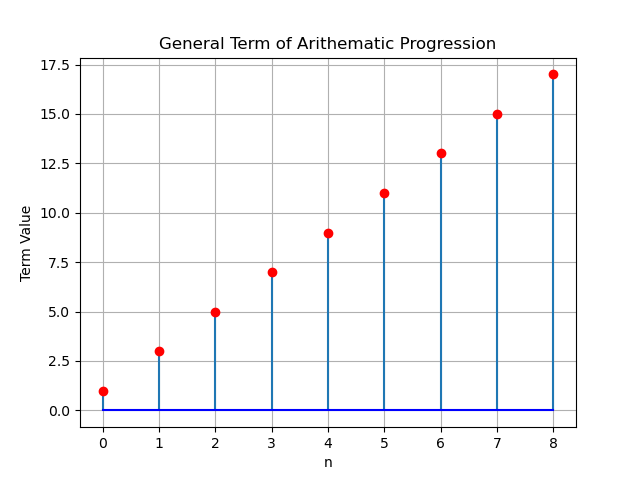
\includegraphics[width=1.0\linewidth]{ncert-maths/11/9/2/16/figs/test.png}
    \caption{Plot of x(n) vs n}
    \label{fig:1}
\end{figure}\\
The Z-Transform is\\
\begin{align}
    X\brak{z}&=2\brak{\dfrac{z}{\brak{z-1}^{2}}}+U\brak{z}\\
    &=\dfrac{2z}{\brak{z-1}^{2}}+\dfrac{1}{1-z^{-1}}\\
    X\brak{z}&=\dfrac{z^2+z}{\brak{z-1}^{2}} \quad{|z|>1}
\end{align}

\pagebreak


\item Check whether -150 is a term of the AP: 11,8,5,2,....

 \solution
 \iffalse
\let\negmedspace\undefined
\let\negthickspace\undefined
\documentclass[journal,12pt,onecolumn]{IEEEtran}
\usepackage{cite}
\usepackage{amsmath,amssymb,amsfonts,amsthm}
\usepackage{algorithmic}
\usepackage{graphicx}
\usepackage{textcomp}
\usepackage{xcolor}
\usepackage{txfonts}
\usepackage{listings}
\usepackage{enumitem}
\usepackage{mathtools}
\usepackage{gensymb}
\usepackage{comment}
\usepackage[breaklinks=true]{hyperref}
\usepackage{tkz-euclide} % loads  TikZ and tkz-base
\usepackage{listings}
\usepackage[latin1]{inputenc}                                
\usepackage{color}                                            
\usepackage{array}                                            
\usepackage{longtable}                                       
\usepackage{calc}                                             
\usepackage{multirow}                                         
\usepackage{hhline}                                           
\usepackage{ifthen}                                           
\usepackage{lscape}
\usepackage{caption}


\newtheorem{theorem}{Theorem}[section]
\newtheorem{problem}{Problem}
\newtheorem{proposition}{Proposition}[section]
\newtheorem{lemma}{Lemma}[section]
\newtheorem{corollary}[theorem]{Corollary}
\newtheorem{example}{Example}[section]
\newtheorem{definition}[problem]{Definition}
%\newtheorem{thm}{Theorem}[section] 
%\newtheorem{defn}[thm]{Definition}
%\newtheorem{algorithm}{Algorithm}[section]
%\newtheorem{cor}{Corollary}
\newcommand{\BEQA}{\begin{eqnarray}}
\newcommand{\EEQA}{\end{eqnarray}}
\newcommand{\define}{\stackrel{\triangle}{=}}
\theoremstyle{remark}
\newtheorem{rem}{Remark}
%\bibliographystyle{ieeetr}

\begin{document}

%
\providecommand{\pr}[1]{\ensuremath{\Pr\left(#1\right)}}
\providecommand{\prt}[2]{\ensuremath{p_{#1}^{\left(#2\right)} }}        % own macro for this question
\providecommand{\qfunc}[1]{\ensuremath{Q\left(#1\right)}}
\providecommand{\sbrak}[1]{\ensuremath{{}\left[#1\right]}}
\providecommand{\lsbrak}[1]{\ensuremath{{}\left[#1\right.}}
\providecommand{\rsbrak}[1]{\ensuremath{{}\left.#1\right]}}
\providecommand{\brak}[1]{\ensuremath{\left(#1\right)}}
\providecommand{\lbrak}[1]{\ensuremath{\left(#1\right.}}
\providecommand{\rbrak}[1]{\ensuremath{\left.#1\right)}}
\providecommand{\cbrak}[1]{\ensuremath{\left\{#1\right\}}}
\providecommand{\lcbrak}[1]{\ensuremath{\left\{#1\right.}}
\providecommand{\rcbrak}[1]{\ensuremath{\left.#1\right\}}}
\newcommand{\sgn}{\mathop{\mathrm{sgn}}}
\providecommand{\abs}[1]{\left\vert#1\right\vert}
\providecommand{\res}[1]{\Res\displaylimits_{#1}} 
\providecommand{\norm}[1]{\left\lVert#1\right\rVert}
%\providecommand{\norm}[1]{\lVert#1\rVert}
\providecommand{\mtx}[1]{\mathbf{#1}}
\providecommand{\mean}[1]{E\left[ #1 \right]}
\providecommand{\cond}[2]{#1\middle|#2}
\providecommand{\fourier}{\overset{\mathcal{F}}{ \rightleftharpoons}}
\newenvironment{amatrix}[1]{%
  \left(\begin{array}{@{}*{#1}{c}|c@{}}
}{%
  \end{array}\right)
}
%\providecommand{\hilbert}{\overset{\mathcal{H}}{ \rightleftharpoons}}
%\providecommand{\system}{\overset{\mathcal{H}}{ \longleftrightarrow}}
        %\newcommand{\solution}[2]{\textbf{Solution:}{#1}}
\newcommand{\solution}{\noindent \textbf{Solution: }}
\newcommand{\cosec}{\,\text{cosec}\,}
\providecommand{\dec}[2]{\ensuremath{\overset{#1}{\underset{#2}{\gtrless}}}}
\newcommand{\myvec}[1]{\ensuremath{\begin{pmatrix}#1\end{pmatrix}}}
\newcommand{\mydet}[1]{\ensuremath{\begin{vmatrix}#1\end{vmatrix}}}
\newcommand{\myaugvec}[2]{\ensuremath{\begin{amatrix}{#1}#2\end{amatrix}}}
\providecommand{\rank}{\text{rank}}
\providecommand{\pr}[1]{\ensuremath{\Pr\left(#1\right)}}
\providecommand{\qfunc}[1]{\ensuremath{Q\left(#1\right)}}
        \newcommand*{\permcomb}[4][0mu]{{{}^{#3}\mkern#1#2_{#4}}}
\newcommand*{\perm}[1][-3mu]{\permcomb[#1]{P}}
\newcommand*{\comb}[1][-1mu]{\permcomb[#1]{C}}
\providecommand{\qfunc}[1]{\ensuremath{Q\left(#1\right)}}
\providecommand{\gauss}[2]{\mathcal{N}\ensuremath{\left(#1,#2\right)}}
\providecommand{\diff}[2]{\ensuremath{\frac{d{#1}}{d{#2}}}}
\providecommand{\myceil}[1]{\left \lceil #1 \right \rceil }
\newcommand\figref{Fig.~\ref}
\newcommand\tabref{Table~\ref}
\newcommand{\sinc}{\,\text{sinc}\,}
\newcommand{\rect}{\,\text{rect}\,}
%%
%       %\newcommand{\solution}[2]{\textbf{Solution:}{#1}}
%\newcommand{\solution}{\noindent \textbf{Solution: }}
%\newcommand{\cosec}{\,\text{cosec}\,}
%\numberwithin{equation}{section}
%\numberwithin{equation}{subsection}
%\numberwithin{problem}{section}
%\numberwithin{definition}{section}
%\makeatletter
%\@addtoreset{figure}{problem}
%\makeatother

%\let\StandardTheFigure\thefigure
\let\vec\mathbf

\bibliographystyle{IEEEtran}

\vspace{3cm}
\title{Assignment}
\author{EE23BTECH11001 - Aashna Sahu}
\maketitle
\bigskip

\renewcommand{\thefigure}{\theenumi}
\renewcommand{\thetable}{\theenumi}
%\renewcommand{\theequation}{\theenumi}
Q:Check whether -150 is a term of the AP: 11,8,5,2,....

 \solution
 \fi

\begin{align}
x(n)&=x(0)+nd\\
n&=\frac{x(n)-x(0)}{d}
\end{align}
\begin{align}
x(n)-x(0) &\equiv 0 \pmod{d}
\end{align}
On substitutings values\\
\begin{align}
-161 &\equiv 2 \pmod{-3}
\end{align}
Thus -150 is not a term of the given AP.
\begin{align}
 \boxed{x(n)=(11-3n)\times u(n)}   
\end{align}

\begin{align}
   X(z)&=\frac{11}{1-z^{-1}}-\frac{3z^{-1}}{(1-z^{-1})^2}\quad
    |z|>1
\end{align}

    \begin{table}[h]
    \centering
    
        \begin{tabular}{|c|c|c|}
	\hline
	\textbf{Symbol} & \textbf{Value} & \textbf{Description} \\[6pt]
	\hline
	$x(0)$ & $25$ & first term of AP \\[6pt]
	\hline
	$d$ & $-3$ & common difference \\[6pt]
	\hline
	$x(n)$ & $(25-3n)u(n)$ & $n$-th term of AP \\[6pt]
	\hline
	$y(n)$ & $116$ & sum of terms \\[6pt]
	\hline 
\end{tabular}

        
    \caption{Input parameters}
    \label{tab:Table10.5.2.6}
\end{table}
\newpage
\begin{figure}[h]
  \centering
  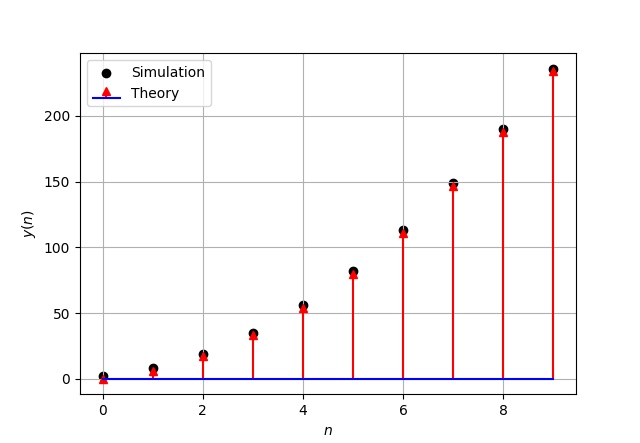
\includegraphics[width=1.2\columnwidth]{ncert-maths/10/5/2/6/figs/Figure_1.png}
  \caption{Representation of x(n)}
  \label{fig:fig10.5.2.6}
\end{figure}
%\end{document}

\pagebreak
\item Find the $12^{th}$ term of a G.P. whose
$8^{th}$ term is $192$ and common ratio is $2$.
\solution
\iffalse
\documentclass[12pt]{article}
\usepackage{amsmath , amssymb}
\usepackage{graphicx}
\usepackage{float}
\usepackage{pgfplots}
\pgfplotsset{compat=1.18}
\newcommand{\tabref}[1]{Table~\ref{#1}}
\newcommand{\figref}[1]{Figure~\ref{#1}}
\providecommand{\abs}[1]{\left\vert#1\right\vert}

\begin{document}

\title{Discrete Assignment}
\author{Mohana Eppala\\ EE23BTECH11018}
\maketitle

\section*{Problem Statement}
Find the value of $n$ so that $\frac{a^{n+1} + b^{n+1}}{a^{n}+b^{n}}$ may be the geometric mean between $a$ and $b$.
\section*{Solution}
\fi
\begin{table}[H]
\centering
\begin{tabular}{|c|c|c|}
        \hline
        \textbf{Parameter} & \textbf{Value} & \textbf{Description} \\
        \hline
	$x(0)$ & $a$ & First term \\
        \hline
	$x(2)$ & $b$ & Third term \\
	\hline
	$x(1)$ & $\sqrt{ab}=\frac{a^{n+1}+b^{n+1}}{a^{n}+b^{n}}$ & Second term\\
	\hline
	$r$ & $\sqrt{\frac{b}{a}}$ & Common ratio \\
	\hline
        $n$ & - & Given variable \\
        \hline
	$x(k)$ & $ar^{k}u(k)$ & General term \\
	\hline
\end{tabular}
\caption{Input parameters table}
\label{tab:11.9.3.27.1}

\end{table}

Consider a GP as in \tabref{tab:1},
\begin{align}
	\therefore \frac{a^{n+1} + b^{n+1}}{a^{n}+b^{n}} &= x(1) \\
	\implies a^{n+1} + b^{n+1} &= a^{n+\frac{1}{2}}b^{\frac{1}{2}} + a^{\frac{1}{2}}b^{n+\frac{1}{2}} \\
\implies a^{n+\frac{1}{2}}(a^{\frac{1}{2}} - b^{\frac{1}{2}}) &= b^{n+\frac{1}{2}}(a^{\frac{1}{2}} - b^{\frac{1}{2}}) \\
\implies (\frac{a}{b})^{n+\frac{1}{2}} &= (\frac{a}{b})^{0} \\
\implies n &= -\frac{1}{2}
\end{align}
From \tabref{tab:1},
\begin{align}
	X(z) &= \frac{a}{1-(\sqrt{\frac{b}{a}})z^{-1}} \quad \abs{z}>\abs{\sqrt{\frac{b}{a}}}
\end{align}
%\end{document}




\end{enumerate}
